
Fig.~\ref{fig:es} shows validation return on 20 fixed seeds against training
time. Both learners passed the PID baseline within about two minutes: ES after
70 generations (2.3\,min) and PPO after \num{500000} environment steps
(1.9\,min). Within the 18.3\,min budget, ES completed 500 generations
(\num{72000} episodes, at most 0.23 billion physics ticks), and PPO collected
4.68 million control steps (37.4 million physics ticks). ES thus consumed up
to about six times as much simulated experience as PPO, but needed no
deep-learning framework at all. Table~\ref{tab:es} compares the final policies
with PID on 100 held-out seeds. We count an episode as a success if the
vehicle does not crash and its mean position error over the last 2\,s is
below 0.25\,m.

\begin{table}[t]
\centering
\caption{Position hold on 100 held-out seeds (random start offset and wind),
after 18.3\,min of CPU-only training. Tail error is the mean position error
over the final 2\,s of an episode.}
\label{tab:es}
\footnotesize
\setlength{\tabcolsep}{4pt}
\begin{tabular}{@{}lcccc@{}}
\toprule
Controller & Return & Tail err.\ (median) & Success & Crash \\
\midrule
Cascaded PID & $-0.433$ & 0.133\,m & 98\% & 0\% \\
ES (NumPy MLP) & $-0.245$ & 0.024\,m & 100\% & 0\% \\
PPO (SB3, PyTorch CPU) & $-0.268$ & 0.024\,m & 100\% & 0\% \\
\bottomrule
\end{tabular}
\end{table}

\begin{figure}[t]
\centering
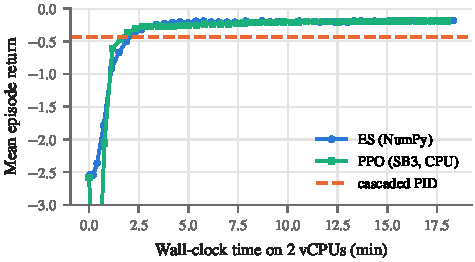
\includegraphics[width=\columnwidth]{fig_es}
\caption{CPU-only training on \skysim: mean validation return on 20 fixed
seeds against wall-clock training time on two vCPUs, for evolution strategies
and PPO, with the cascaded PID baseline for reference. The vertical axis is
clipped at $-3$; PPO's first evaluation after initialisation reached $-5.0$.}
\label{fig:es}
\end{figure}

The two learned policies reach the same median tail error, 0.024\,m, and
neither crashed. The ES policy has the slightly better mean return on the
held-out seeds. The ES and PID results come from one run on the 2.1\,GHz
machine of Section~\ref{sec:eval}; the PPO run was made later on a 2.3\,GHz
vCPU of the same family. Each learner was run with a single seed, so the
comparison between them is indicative only.

This experiment is not a claim that learned policies beat PID control in
general. The PID gains were tuned by hand in a few minutes, and the baseline
has no horizontal integral action, so most of its residual error is the
steady offset caused by wind. A PID controller with wind integrators would
close much of the gap. The claim the experiment supports is narrower: with
either a gradient-free or a standard deep-RL learner, a closed-loop flight
policy can be trained from scratch against \skysim's full rotor model on a
commodity CPU in minutes, without a GPU.
